% !TEX root = root.tex
\chapter{Software Development: A Modern Particle-Tracking Toolkit}
\chaptermark{Software}

A large portion of my thesis effort has been devoted to the development of particle tracking and data analysis software, used for my own soft matter research and the work of others in our group. It is also being adopted by other soft matter researchers at Harvard, Princeton, Oxford, U. Chicago, U. Penn, and more. Relying on the growing open-source scientific software community, I have leveraged free, widely-used code for core functionality. By contributing my own particle tracking and data analysis code back to the community, I have increased the impact of the work and encouraged others to share their own improvements to my code, from which all users benefit.

One fast-growing product of this community is the notebook, a standard, browser-based record of code with figures, explanatory text and equations, and links and references. As recently outlined in an article published in \emph{Nature}\cite{Shen2014}, notebooks are making data analysis easier to record, understand, and reproduce. Many authors are publishing notebooks alongside papers, providing the the detail that is essential for others to reproduce the work in a reasonable time scale.

\section{Introduction}

Particle tracking is an extremely powerful technique used across many disciplines of science. It has been used to directly image atomic rearrangements in silica glass\cite{Huang2013a}; to image stress and strain in drying colloidal films\cite{Xu2013a}; to image pleats in crystals on curved surfaces\cite{Irvine2010}; to [add biophys. examples].

\section{Review of the Crocker--Grier Particle Tracking Algorithm}

The particle tracking algorithm implemented by Crocker and Grier is performed in two steps: locating the particles in each frame and identifying the particles through time, linking coordinates into trajectories.

Trackpy implements the tracking algorithm of Crocker and Grier\cite{Crocker1996}. Theirs and similar algorithms\cite{Ghosh1994} have been widely used in the fields of colloid science, microrheology, biophysics, and biometrical engineering. The Crocker and Grier algorithm was originally implemented in the IDL programming language, but it has since been translated into various other languages, including Python, MATLAB, and C++. (A list of these related projects is maintained in the Trackpy Documentation in Appendix A.) Numerous alternative algorithms have been developed for tracking particles, which we discuss later.

In the algorithm of Crocker and Grier, particle coordinates are identified in four steps: 1) preparing the image using common image-processing techniques; 2) finding local maxima of brightness that may correspond to particles; 3) honing in on each candidate particle�s exact center with subpixel precision; and 4) discerning which of the candidates are true particles based on their morphology and measured brightness.

The software first prepares the images by applying a spatial bandpass filter, which uses a Fourier transform of the image to suppress features with small-scale variation (e.g., camera noise) and large-scale variation (e.g., uneven lighting). This effectively erases any objects in the background that are much smaller or much larger than the size of the particles. Next, the software identifies all local maxima in the processed image. These do not necessarily correspond to the particles' centers, but they provide an initial estimate of where particles may be found. If two or more local maxima are separated by a distance smaller than the particle diameter, they are assumed to belong to the same particle, and the software only retains the brightest one. Then, the software finds the intensity-weighted centroid (``center of mass'') of each spot, which is refined through iterative steps, using the whole region of the particle to resolve its center to a precision much better than 1 pixel. Finally, the software characterizes the neighborhood surrounding each spot by its total brightness, size, and eccentricity (deviation from circular shape). Using these attributes, spots that correspond to actual particles can be distinguished -- and the rest discarded -- with minimal user input. For example, true particles tend to appear bright and circular.

At this point, the software has identified the locations of particles in each frame. Next, the locations must be linked together across frames into particle trajectories. The algorithm robustly handles the complications of real trajectories: Particles are allowed to leave the frame, new particles are allowed to enter, and particles can even be tracked if they temporarily vanish and reappear nearby within a user-specified number of frames. If particles are well separated and moving slowly relative to the frame rate, the task of linking them is simple and unambiguous. If there are many particles in the field of view and they are moving quickly, the Crocker and Grier linking algorithm assigns particles in a way that minimizes the total length of the links. This is grounded in the statistics of random walks; a Brownian particle is most likely to be found near where it was last seen. The linking algorithm is rigorously correct for non-interacting Brownian particles [Crocker and Grier], and it is employed effectively in a variety of tracking applications. (See Section 4.3.2 for a more on trajectory linking.)

As the number of particles in view grows, resolving ambiguous networks is difficult. To simplify the problem, the algorithm requires the user to specify the maximum displacement allowed from one frame to the next. A good choice can simply be obtained by watching the particles and guessing the upper range of their movement between frames. For Brownian motion, the Stokes-Einstein equation provides a guideline as well. After trajectory linking is complete, inspect a histogram of displacements at the shortest time scale. If the histogram decays to zero just before the maximum displacement, then the choice of maximum displacement was proper. However, if the histogram stops abruptly at the maximum displacement, then redo trajectory linking with a larger maximum displacement. If, on the other hand, few displacements are nearly as large as the specified maximum displacement, then it may be set lower for better performance and accuracy.

To process a set of videos with automated tracking, only a few minutes of user attention are required to input parameters and check that they are suitable. A standard computer will typically be able to process at least one video frame per second, though this depends on the number of particles (and therefore the number of calculations needed for a single frame) in the video, as well as the exact automated tracking algorithm and implementation used. Thus, the software can process a typical video of a few hundred frames in a few minutes. The code will output the trajectories in a text file, spreadsheet, or database. Subsequent data analysis will depend on the scientific question under investigation. We discuss data analysis strategies in Section 3.3. 


\section{Particle Tracking in Trackpy}

A more detailed walkthrough in included among the extensive documentation and examples in the Appendix A.

\section{Subpixel precision and accuracy}

Understanding the precision and accuracy of particle localization is critical for conducting reliable particle tracking experiments. In fact, failure to recognize and account for imprecision and inaccuracy in tracking data can lead to misinterpretation (Deschout 2014; Parthasarathy). Precision refers to uncertainty in location, and is defined as the standard deviation of the measured locations when a single stationary particle is imaged and localized multiple times. In contrast, accuracy describes whether the position estimates deviate from the true particle position with systematic bias (Cheezum; Deschout). 

Tracking resolution (i.e., localization precision) is different than microscope resolution. As classically defined, microscope resolution is the minimum distance between two distinguishable points. The resolution of a traditional light microscope is approximately 250 nm, half the wavelength of visible light (Thompson). However, this limit does not apply to locating the center of one isolated point. Using an appropriate algorithm, it is possible to localize the center of an isolated particle or point source to better than the diffraction-limited resolution (Bobroff; Deschout 2014). In fact, researchers can routinely track particles with a lateral spatial precision of tens of nanometers or less using a standard light microscope (Crocker and Hoffman).
How is it possible to locate a particle�s center to better than pixel resolution? If a particle is only visible as one bright pixel, then we can only say that the particle is located somewhere in that pixel. But if the particle�s image spans multiple pixels -- ideally, more than three pixels across -- we can find its position with subpixel accuracy by taking the average position of these pixels, weighted by brightness. Alternative methods for calculating particle position with subpixel resolution are discussed in Section X.

\subsection{Static Error}

Tracking precision is subject to both fundamental and experimental limitations. The fundamental limitation is photon noise: a particle emits photons stochastically, and consequently, there is statistical uncertainty in locating the particle from its image (Fig. 9 and Table 1) (Ober). The size of this uncertainty is inversely proportional to the square root of the number of detected photons (Ober; Crocker).
Experimental limitations related to detector and specimen properties can also degrade localization precision. Detector noise, including dark current (thermally-induced electrons in the detector) and readout noise (errors in reading the number of photoelectrons built up in a pixel), can interfere with particle localization (Thompson; Deschout). Detector noise is greatly reduced in high-performance, cooled, EMCCD cameras. Specimen autofluorescence and out-of-focus background fluorescence can also reduce localization precision and accuracy, which can be an issue when tracking particles in a thick biological specimen using standard epifluorescence illumination. Image processing can remove some, but not all, of this background (Deschout 2014). Finally, lateral localization precision of fluorescent particles is best for particles located in the focal plane -- where the particle image is smallest, brightest, and closest to a Gaussian curve in shape -- and decreases with increasing distance from the focal plane (Savin 2008; Deschout 2014).
This inability to exactly localize particles has been referred to as static error, localization error, or random error (Savin and Doyle; Martin; Crocker). Static error adds a constant offset to the MSD, as derived previously (Martin): $\langle \Delta r^2 \rangle + 2*\epsilon^2$, where $\epsilon$ is the localization uncertainty. A perfectly immobilized particle will have a true MSD = 0 for all lag times, but because of static error, the actual measured MSD will be a non-zero constant, $\langle \Delta r^2 \rangle = 2*\sigma^2$ (Martin; Crocker). However, in most particle tracking experiments, the true underlying MSD is not known a priori, so it may not be immediately evident which component of the measured MSD is �true" and which is artifact.
In addition to the random error associated with camera noise and pixelation, particle localization is subject to systematic errors, wherein particles can be �biased� toward certain locations, such pixel centers. Several experimental details in both hardware and software are implicated in these errors (Crocker and Hoffman again). Of course, if the particles typically step much more than a pixel between frames, optimizing subpixel resolution is less important. Readers with applications where particles frequently move in subpixel steps are encouraged to consult the referenced literature and consider these details with care.

\subsection{Dynamic Error}

Additional error is introduced by motion blur. When a particle moves substantially during the camera exposure time, a blurred spot is recorded, representing the time integral of the particle�s location (Fig. 10 and Table 1). Particle motion during the exposure time reduces the observed MSD at short times for randomly diffusing particles, since they tend to revisit previously explored regions (Crocker and Hoffman; Berg). This effect has been called dynamic error (Savin and Doyle). In addition, particle motion increases static error, because motion blur reduces localization precision by roughly two-fold under typical experimental conditions, as compared to stationary particles (Deschout 2012).
Like static error, dynamic error can alter the measured MSD, and can thus introduce inaccuracies when using the MSD to calculate diffusion coefficients and viscoelastic moduli. Static error alone adds a constant offset to the MSD, which flattens the MSD at short time scales on a log-log plot, and makes diffusive motion appear sub-diffusive (Martin). Dynamic error, by itself, decreases the MSD at short time scales, which makes diffusive motion appear like active transport. Static and dynamic error act in opposite directions, so depending on which type of error is larger, one effect may dominate, or occasionally, the two effects may largely cancel each other (Savin and Doyle). Both sources of error are more pronounced at short time scales, when the true MSD is smaller.

\subsection{Experimental Best Practices to Minimize Error}
Prior to collecting data, it is critical that researchers consider how to minimize static and dynamic error, as they are difficult if not impossible to completely correct after the experiment. To boost signal-to-noise ratio and reduce static error, researchers should choose bright particles, a microscope objective with large numerical aperture, and a sensitive camera with low noise. The only way to reduce dynamic error is to use an exposure time that is small compared to the frame interval (Savin and Doyle; Crocker and Hoffman). Unfortunately, shorter exposure time also increases static error. A compromise is to use the longest exposure time possible without introducing large dynamic error. As a point of reference, for Brownian motion, an exposure time no longer than one quarter the frame interval will cause dynamic error of <10\% at the shortest time scale, and smaller dynamic error at longer time scales (Crocker and Hoffman).
After conducting an experiment, dynamic error is especially difficult to correct, because it is time-dependent and also depends on the underlying type of motion, which is often unknown (Savin and Doyle). Static error is simpler to quantify and correct ex post facto, since static error adds a constant offset to MSD regardless of the nature of particle motion. Static error can be estimated by tracking particles fixed to a coverslip under signal-to-noise conditions similar to those of the experiment, and then subtracted from the ensemble MSD. However, this simple approach may not precisely mimic the background noise in the experiment, nor the effect that motion blur has on static error. An alternative method has recently been proposed for measuring localization precision of moving particles, though this technique requires a custom microscope configuration (Deschout 2012). Tracking particles in water or other fluids of known viscosity and comparing their MSD to theory may also help reveal types and magnitudes of error. 
How much do researchers conducting particle tracking experiments need to worry about static and dynamic error? The answer depends both on the system under investigation and on the desired analysis. If the research objective is to precisely quantify diffusion coefficients or viscoelastic moduli, or to fit the data to a model, it is critical to consider error to ensure proper analysis -- especially if the imaging conditions were not ideal. In particular, higher spatial and temporal resolution are needed to accurately study particle motion at short times scales, where the MSD is smaller and the errors proportionally larger. However, if the research objective is to qualitatively compare the transport of two types of nanoparticles with very different behavior, such as mobile and immobile, moderate tracking errors require less thorough examination and are unlikely to alter the final conclusion. 

\section{Prediction Framework}

The Crocker--Grier particle tracking algorithm, at its simplest level, takes each particle in
the previous frame and tries to find it in the current frame. This
requires knowing where to look for it. The algorithm was developed to track particles undergoing Brownian diffusion,
in which a particle's velocity is uncorrelated from one
frame to the next. Therefore, a particle is statistically most likely to be found at or near is last known location. The particle in the current frame closet to a particle in the previous frame is likely to be the same particle.

Let's formalize this guessing as \emph{prediction}. Consider a function

\begin{equation}
P(t_1, t_0, \vec x(t_0))
\end{equation}

\noindent that takes the particle at position $\vec x(t_0)$ and predicts its
future position $\vec x(t_1)$. The optimal predictor for Brownian motion
is

\begin{equation}
P(t_1, t_0, \vec x(t_0)) = \vec x(t_0)
\end{equation}

\noindent which, of course, is also the simplest to implement.

The better our prediction about where to look in the next frame, the
more likely we will find the one and only particle we seek.
In practice, the algorithm looks for the particle in a circular region of radius
\texttt{search\_range}, centered on $P(t_1, t_0, \vec x(t_0))$. So to
successfully track particle $i$ puts a limit on the error in our
prediction:

\begin{equation}
\label{eqn:brownian-predictor}
\|P(t_1, t_0, \vec x_i(t_0)) - \vec x_i(t_1)\| \le \tt{search\_range}
\end{equation}

This favors a generous \texttt{search\_range}. However, if
\texttt{search\_range} is too big, then for each particle in the
previous frame there will be many possible matches in the current frame,
and so matching one frame to the next requires the computer to evaluate
an overwhelming set of possibilities, seeking the one that minimizes the total displacements of all particles. Tracking may become extremely
slow, the problem effectively intractable.
So for the Brownian $P$ above, \texttt{search\_range} must be bigger
than the largest particle displacement between frames, but smaller than
the typical spacing between particles\cite{Crocker1996}. If such a value does not exist, the Crocker--Grier algorithm is not effective.

However, if particle motion is not strictly Brownian, its velocity
probably \emph{is} correlated in time. We may be able to improve $P$. This 
is the justification for trackpy's prediction feature.

\subsection{Prescribed predictors}\label{prescribed-predictors}

Consider a toy example: a regular array of particles,
translating with constant velocity $v$. Figure \ref{fig:prediction-const-features}
shows the particles' positions in two consecutive frames.

    \begin{figure}
    \centering
    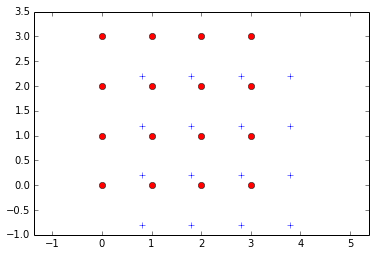
\includegraphics[width=\columnwidth]{prediction/prediction_4_1}
    \caption{\label{fig:prediction-const-features}An ensemble of particles moving under constant velocity. The red circles represent their positions at some time $t$, the blue crosses at some later time $t'$.}
    \end{figure}

\noindent Using the Brownian predictor, Eq. (\ref{eqn:brownian-predictor}), trackpy links the particles as shown in Figure \ref{fig:prediction-const-brownian-link}.

   \begin{figure}
    \centering
    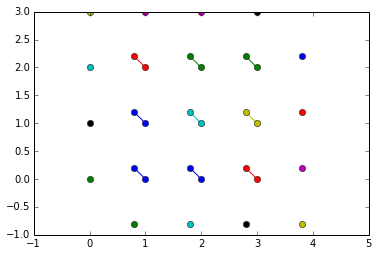
\includegraphics[width=\columnwidth]{prediction/prediction_7_0}
    \caption{\label{fig:prediction-const-brownian-link}An ensemble of particles moving under constant velocity are identified through time using a simple Brownian prediction, Eq. (\ref{eqn:brownian-predictor}). Features that have been identifies as belonging to the same trajectory are connected by a line. In this case, the identification is not correct.}
    \end{figure}
    
\noindent This is obviously not correct. Let us provide a $P$ which reflects this constant

\begin{equation}
\label{eqn:const-predictor}
P(t_1, t_0, \vec x_i(t_0)) = \vec x_i(t_0) + v(t_1 - t_0)
\end{equation}

\noindent The result is accurate (Figure \ref{fig:prediction-const-const-link}). To be clear, the predictor does not need to specify exactly where the
particle will be; it only must bias the search enough that the correct
identification will be made.

   \begin{figure}
    \centering
    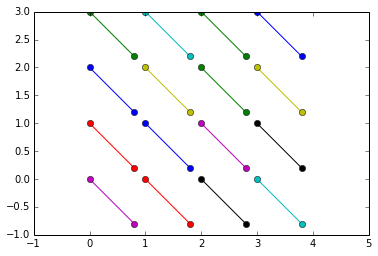
\includegraphics[width=\columnwidth]{prediction/prediction_9_1}
    \caption{\label{fig:prediction-const-const-link}An ensemble of particles moving under constant velocity are identified through time using a constant-velocity predictor, Eq. (\ref{eqn:const-predictor}). Features that have been identifies as belonging to the same trajectory are connected by a line.}
    \end{figure}

\subsection{Dynamic predictors}\label{dynamic-predictors}

In typical experimental conditions, the particles' velocities are not known ahead of time. It would be much better for the predictor to ``learn'' about
the velocities, and allow different particles to have different
velocities that can change over time. To accomplish this, $P$ will depend on more than $x_0$, $t_0$, and $t_1$; it will also depend on the particles' most recent velocities.

\begin{equation}
\label{eqn:adaptive-predictor}
P(t_1, t_0, \vec x_i(t_0)) = \vec x_i(t_0) + \frac{\vec x_i(t_0) - \vec x_i(t_{-1})}{t_0 - t_{-1}} (t_1 - t_0)
\end{equation}

There are a few caveats.
  If a new particle is in frame $t_i$ but wasn't in $t_{i-1}$, its velocity is unknown, but it is estimated using the velocity of the nearest existing particle. Of course, in the first frame, all
  velocities are unknown because
  there is no previous frame. Fortunately, even though particles may be in motion from the start, an initial guess
  of $v_0 = 0$ often gives acceptable results. In many cases, at
  least some of the particles are moving slowly enough that they can be
  tracked and their velocity can be obtained. Then, because particles with
  unknown velocity borrow the nearest known velocity, this may give the algorithm a foothold to track more particles
  in later frames. If that is not sufficient, a more accurate initial guess can be specified. This guess can be a constant velocity, a velocity profile, or N-dimensional velocity field.

As a demonstration, consider a three-frame sequence that starts
with small displacements and accelerates. With a simple Brownian predictor, tracking fails at the third frame (Figure \ref{fig:prediction-acceleration-brownian-link}). With the adaptive predictor, Eq. (\ref{eqn:adaptive-predictor}), tracking is accurate (Figure \ref{fig:prediction-acceleration-adaptive-link}).


   \begin{figure}
    \centering
    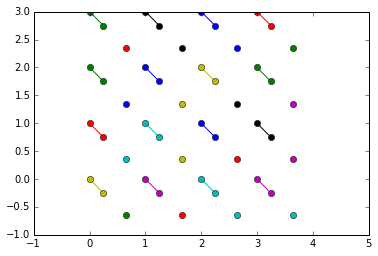
\includegraphics[width=\columnwidth]{prediction/prediction_14_1}
    \caption{\label{fig:prediction-acceleration-brownian-link}An ensemble of accelerating particles are identified through time using a simple Brownian prediction, Eq. (\ref{eqn:brownian-predictor}). The identification is incorrect.}
    \end{figure}
   

   \begin{figure}
    \centering
    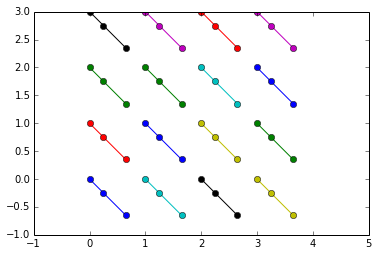
\includegraphics[width=\columnwidth]{prediction/prediction_16_1}
    \caption{\label{fig:prediction-acceleration-adaptive-link}An ensemble of accelerating particles are identified through time using a simple Brownian prediction, Eq. (\ref{eqn:adaptive-predictor}).}
    \end{figure}


    \subsubsection{Channel flow prediction}\label{channel-flow-prediction}

There are two special cases implemented by trackpy. The first is channel flow, in which velocities are relatively uniform in one
direction. For example, if the channel is in the $x$ (i.e. $\hat i$)
direction, particle velocities are very well approximated as

\begin{equation}
\vec v = \hat i v_x(y)
\end{equation}

\noindent where the velocity profile $v_x(y)$ is a smoothly-varying function
defined across the channel. The required inputs are the direction of flow and size of the bins used to
define the channel profile. The initial velocities can be specified or arrived at adaptively.

Figure \ref{fig:prediction-channel-brownian-link} shows an example. The simple Brownian prediction fails for the top row of particles at the edge of the channel. With a Channel Flow prediction, the tracking is accurate (Figure \ref{fig:prediction-channel-channel-link}).

   \begin{figure}
    \centering
    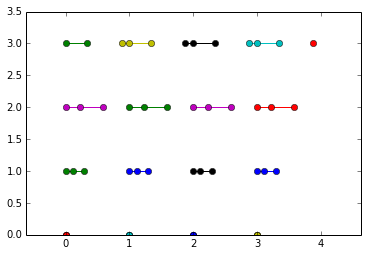
\includegraphics[width=\columnwidth]{prediction/prediction_20_1}
    \caption{\label{fig:prediction-channel-brownian-link}An ensemble of particle moving in simulated channel flow are identified through time using a simple Brownian prediction, Eq. (\ref{eqn:brownian-predictor}). The identification is incorrect.}
    \end{figure}

   \begin{figure}
    \centering
    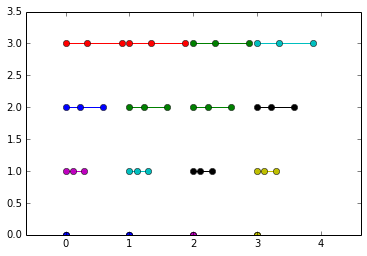
\includegraphics[width=\columnwidth]{prediction/prediction_22_1}
    \caption{\label{fig:prediction-channel-channel-link}An ensemble of particle moving in simulated channel flow are identified through time using a Channel Flow predictor.}
    \end{figure}
   

    \subsubsection{Drift prediction}\label{drift-prediction}
    
The second special case implemented by trackpy is drift prediction. At the interface, it is common to observed convective flows driven by air currents or heat from the illuminating lamp. In the final data analysis, this motion can often be subtracted away by adopting a reference frame set by the average velocity of the ensemble of particles. Likewise, tracking accuracy and performance is improved by forming a prediction based on the average velocity of the ensemble.

\section{Results}
\subsection{Accuracy vs. ``ground truth'' and vs. other approaches}
\subsection{Performance}
\section{Testing \& Reproducibility}

Trackpy is packaged with more than 150 automated tests: snippets of code that exercise a specific capability of trackpy by running toy examples and comparing the output to known correct results. For example, to test feature location, an automated test draws a simple image with several dots and checks that trackpy can locate the dots with a given precision.

Testing benefits a research code in more than one way. Most obviously, tests verify correctness and check special cases. Just as important, tests protect reproducibility. By codifying key results as tests, authors can be sure that these results cannot be broken inadvertently in the future. This empowers users who do not have familiarity with the whole codebase to make contributions and changes with confidence that they will not have unintended consequences. When revisions are submitted to trackpy, a web service automatically executes all the tests, and it alerts the user if any tests fail under the proposed change. Finally, the test suite complements the documentation. Technical users and potential contributors can browse it as a comprehensive demonstration of the ways in which the authors imagined the code would be used.

Trackpy has an unusual level of testing for a code from an academic lab. But the time invested has been worthwhile: it ensures that any research that depends on the code is grounded in a rigorous, scientific approach to software development. This gauruntee earns the confidence of other researchers who decide to use, cite, or contribute to the codebase. It thereby increases the code's longevity and the impact of the development effort.

As trackpy is improved and changed, old research code may cease to reproduce exactly the same results. Testing help ensure that any such "breaking changes" are made deliberately and can be documented. To avoid breaking old code altogether, researchers can make note of which specific version of trackpy was used for a given project and roll back to that version when revisiting the research. Several new projects such as Docker, Dexy, and hashdist [any academic citations for these?] address this need: they recreate complete computing environments, making it possible reproduce research using the specific original versions of all the relevant software. These tools are especially powerful in simulation research, where the entire research project can reproduced on a computer. But they are also useful in experimental science, covering every step after data collection up to the production of the published figure.

\section{Conclusion}
\subsection{``A Modern Approach''}
Trackpy is distinguished among niche academic codes by its careful adherence to the best practices of the open source software community. The most important are code review and open discussion before each revision, automated testing, complete API documentation. Also, code comprehensibility and modularity are key design considerations. Code that merely works is not necessarily easy to test, maintain, extend, or reuse.

Code for academic use is typically developed for a single research project, often by a single researcher, at least at first. Trackpy has benefitted from its co-development by three different researchers working in separate groups at separate institutions on projects with vastly different priorities. The core functionality of trackpy was useful to all, and the healthy tension in the project drove the development of extensible, reusable code. In addition to the core developers, collaborators and undergraduate researchers used trackpy actively during its development. Their use of the cutting-edge code demanded stability and thorough documentation. As the project matured, a wider community of users discovered it and found it useful.

\subsection{Measuring Success}
The scientific software community has not settled on a single metric for the success of academic software. In the three years since the first lines of code were written, trackpy has supported published research from several academic research groups; trackpy has been downloaded thousands of times through the Python Package Index, though it is impossible to know if the recipients were genuine users; trackpy has been adopted by users from about ten top academic research institutions known to the authors. Most importantly, trackpy has benefitted from code contributions offered by those users, comprising both software experts and relative novices.

Particle tracking is a general problem in a number of fields, and thanks to the pioneering efforts of John Crocker, David Grier, and Eric Weeks, it has a strong tradition of open source code supporting first-rate research.

\subsection{Future Directions}

Trackpy can increase its impact and extend its applicability by incorporating algorithms and strategies from outside the colloids literature and the software lineage of Crocker and Grier. Researchers in the biological and biophysics communities also use these tools, but they have developed additional methods to solve richer problems. For example, in biological contexts, features must be located amidst a complex, busy environment where they are more difficult to distinguish and the methods discussed above can be insufficient to extract them. Tracking and the notion of a trajectory can be subtler, as features might split or merge with each other.

Separately, the scientific Python community continues to grow and develop ever more powerful tools for exploring, processing, and presenting data. Trackpy will build on this ongoing progress, providing tools specific to the needs of particle tracking.